
% Programming/Coding Assignment
% LaTeX Template
%
% This template has been downloaded from:
% http://www.latextemplates.com
%
% Original author:
% Ted Pavlic (http://www.tedpavlic.com)
%
% Note:
% The \lipsum[#] commands throughout this template generate dummy text
% to fill the template out. These commands should all be removed when 
% writing assignment content.
%
% This template uses a Perl script as an example snippet of code, most other
% languages are also usable. Configure them in the "CODE INCLUSION 
% CONFIGURATION" section.
%
%%%%%%%%%%%%%%%%%%%%%%%%%%%%%%%%%%%%%%%%%

%----------------------------------------------------------------------------------------
%   PACKAGES AND OTHER DOCUMENT CONFIGURATIONS
%----------------------------------------------------------------------------------------

\documentclass{article}

\usepackage{fancyhdr} % Required for custom headers
\usepackage{lastpage} % Required to determine the last page for the footer
\usepackage{extramarks} % Required for headers and footers
\usepackage[usenames,dvipsnames]{color} % Required for custom colors
\usepackage{graphicx} % Required to insert images
\usepackage{listings} % Required for insertion of code
\usepackage{courier} % Required for the courier font
\usepackage{lipsum} % Used for inserting dummy 'Lorem ipsum' text into the template
\usepackage{multicol}
\usepackage{fullpage,amsthm,amsfonts,amssymb,epsfig,amsmath}
\usepackage{tikz}
\usepackage{verbatim,array}
\usepackage[active,tightpage]{preview}
\usetikzlibrary{decorations.pathmorphing,shapes,positioning,calc,fit,arrows,arrows.meta}
\setlength\PreviewBorder{5pt}

\usepackage{scrextend}
\newcommand{\tikzmark}[1]{%
  \tikz[overlay,remember picture] \node(#1){};
}

% Margins
\topmargin=-0.45in
\evensidemargin=0in
\oddsidemargin=0in
\textwidth=6.5in
\textheight=9.0in
\headsep=0.25in

\linespread{1.1} % Line spacing

% Set up the header and footer
\pagestyle{fancy}
\lhead{\hmwkAuthorName} % Top left header
\chead{\hmwkClass\ (\hmwkClassInstructor\ \hmwkClassTime): \hmwkTitle} % Top center head
\rhead{\firstxmark} % Top right header
\lfoot{\lastxmark} % Bottom left footer
\cfoot{} % Bottom center footer
\rfoot{Page\ \thepage\ of\ \protect\pageref{LastPage}} % Bottom right footer
\renewcommand\headrulewidth{0.4pt} % Size of the header rule
\renewcommand\footrulewidth{0.4pt} % Size of the footer rule
\newcommand{\tab}{\hspace*{3em}}

\setlength\parindent{0pt} % Removes all indentation from paragraphs

%----------------------------------------------------------------------------------------
%   CODE INCLUSION CONFIGURATION
%----------------------------------------------------------------------------------------

\definecolor{MyDarkGreen}{rgb}{0.0,0.4,0.0} % This is the color used for comments
\lstloadlanguages{Perl} % Load Perl syntax for listings, for a list of other languages supported see: ftp://ftp.tex.ac.uk/tex-archive/macros/latex/contrib/listings/listings.pdf
\lstset{language=Perl, % Use Perl in this example
        frame=single, % Single frame around code
        basicstyle=\small\ttfamily, % Use small true type font
        keywordstyle=[1]\color{Blue}\bf, % Perl functions bold and blue
        keywordstyle=[2]\color{Purple}, % Perl function arguments purple
        keywordstyle=[3]\color{Blue}\underbar, % Custom functions underlined and blue
        identifierstyle=, % Nothing special about identifiers                                         
        commentstyle=\usefont{T1}{pcr}{m}{sl}\color{MyDarkGreen}\small, % Comments small dark green courier font
        stringstyle=\color{Purple}, % Strings are purple
        showstringspaces=false, % Don't put marks in string spaces
        tabsize=5, % 5 spaces per tab
        %
        % Put standard Perl functions not included in the default language here
        morekeywords={rand},
        %
        % Put Perl function parameters here
        morekeywords=[2]{on, off, interp},
        %
        % Put user defined functions here
        morekeywords=[3]{test},
        %
        morecomment=[l][\color{Blue}]{...}, % Line continuation (...) like blue comment
        numbers=left, % Line numbers on left
        firstnumber=1, % Line numbers start with line 1
        numberstyle=\tiny\color{Blue}, % Line numbers are blue and small
        stepnumber=5 % Line numbers go in steps of 5
}

% Creates a new command to include a perl script, the first parameter is the filename of the script (without .pl), the second parameter is the caption
\newcommand{\perlscript}[2]{
\begin{itemize}
\item[]\lstinputlisting[caption=#2,label=#1]{#1.pl}
\end{itemize}
}

%----------------------------------------------------------------------------------------
%   DOCUMENT STRUCTURE COMMANDS
%   Skip this unless you know what you're doing
%----------------------------------------------------------------------------------------

% Header and footer for when a page split occurs within a problem environment
\newcommand{\enterProblemHeader}[1]{
\nobreak\extramarks{#1}{#1 continued on next page\ldots}\nobreak
\nobreak\extramarks{#1 (continued)}{#1 continued on next page\ldots}\nobreak
}

% Header and footer for when a page split occurs between problem environments
\newcommand{\exitProblemHeader}[1]{
\nobreak\extramarks{#1 (continued)}{#1 continued on next page\ldots}\nobreak
\nobreak\extramarks{#1}{}\nobreak
}

\setcounter{secnumdepth}{0} % Removes default section numbers
\newcounter{homeworkProblemCounter} % Creates a counter to keep track of the number of problems

\newcommand{\homeworkProblemName}{}
\newenvironment{homeworkProblem}[1][Problem \arabic{homeworkProblemCounter}]{ % Makes a new environment called homeworkProblem which takes 1 argument (custom name) but the default is "Problem #"
\stepcounter{homeworkProblemCounter} % Increase counter for number of problems
\renewcommand{\homeworkProblemName}{#1} % Assign \homeworkProblemName the name of the problem
\section{\homeworkProblemName} % Make a section in the document with the custom problem count
\enterProblemHeader{\homeworkProblemName} % Header and footer within the environment
}{
\exitProblemHeader{\homeworkProblemName} % Header and footer after the environment
}

\newcommand{\problemAnswer}[1]{ % Defines the problem answer command with the content as the only argument
\noindent\framebox[\columnwidth][c]{\begin{minipage}{0.98\columnwidth}#1\end{minipage}} % Makes the box around the problem answer and puts the content inside
}

\newcommand{\homeworkSectionName}{}
\newenvironment{homeworkSection}[1]{ % New environment for sections within homework problems, takes 1 argument - the name of the section
\renewcommand{\homeworkSectionName}{#1} % Assign \homeworkSectionName to the name of the section from the environment argument
\subsection{\homeworkSectionName} % Make a subsection with the custom name of the subsection
\enterProblemHeader{\homeworkProblemName} % Header and footer within the environment
}{
\enterProblemHeader{\homeworkProblemName} % Header and footer after the environment
}

%----------------------------------------------------------------------------------------
%   NAME AND CLASS SECTION
%----------------------------------------------------------------------------------------

\newcommand{\hmwkTitle}{Homework\ \#7} % Assignment title
\newcommand{\hmwkDueDate}{Tuesday,\ May\ 26th,\ 2015} % Due date
\newcommand{\hmwkClass}{CMPS\ 102} % Course/class
\newcommand{\hmwkClassTime}{4:00pm} % Class/lecture time
\newcommand{\hmwkClassInstructor}{Warmuth} % Teacher/lecturer
\newcommand{\hmwkAuthorName}{John Allard \ 1437547
} % Your name


%----------------------------------------------------------------------------------------
%----------------------------------------------------------------------------------------
%   USER SETTINGS
%----------------------------------------------------------------------------------------
%----------------------------------------------------------------------------------------
\usepackage{mathtools}
\DeclarePairedDelimiter\ceil{\lceil}{\rceil}
\DeclarePairedDelimiter\floor{\lfloor}{\rfloor}



%----------------------------------------------------------------------------------------
%   TITLE PAGE
%----------------------------------------------------------------------------------------

\title{
\vspace{2in}
\textmd{\textbf{\hmwkClass:\ \hmwkTitle}}\\
\normalsize\vspace{0.1in}\small{Due\ on\ \hmwkDueDate}\\
\vspace{0.1in}\large{\textit{}}
\vspace{3in}
}

\author{\textbf{\hmwkAuthorName}}
\date{} % Insert date here if you want it to appear below your name

%----------------------------------------------------------------------------------------

\begin{document}

\maketitle

%----------------------------------------------------------------------------------------
%   TABLE OF CONTENTS
%----------------------------------------------------------------------------------------

%\setcounter{tocdepth}{1} % Uncomment this line if you don't want subsections listed in the ToC

% \tableofcontents
\newpage





%----------------------------------------------------------------------------------------
%   PROBLEM 1
%----------------------------------------------------------------------------------------

% To have just one problem per page, simply put a \clearpage after each problem

\begin{homeworkProblem}
1) Consider the longest common subsequence problem between two strings $x_1,...,x_n$ and $y_1,...,y_m$. Define a graph over the nxm grid (plus possibly some vertices around the edges) s.t. the longest common subsequence corresponds to the longest path in this graph.
- Clearly describe the condition for the presence of an edge between two vertices on the grid. \\
- How should the edges be labeled? \\
- How do you find the longest path? \\
- Is this algorithm more efficient than the dynamic programming algorithm? \\

\textbf{Answer : }
We will solve this problem using a directed graph over $m \times n$ vertices that are labeled according to their coordinates $(p,q)$ : $0 \leq p \leq m$ and $0 \leq q \leq n$. Edges are generated as follows :
if letters $p$ and $q$ are the same, draw an edge from $V(p, q)$ to $V(p+1, q+1)$, aka a diagonal. If the letters are different, draw two edges from $V(p, q)$, one to $V(p+1, q)$ and the other to $V(p, q+1)$, aka down and right. The import part is this : edges that go diagonal are given a weight of 1, and edges that go right or down get a weight of 0. The longest path now doens't depend on the number of edges directly, but rather how many diagonal edges are along a path, since they contribute all of the weight.  \\

\begin{multicols}{2}
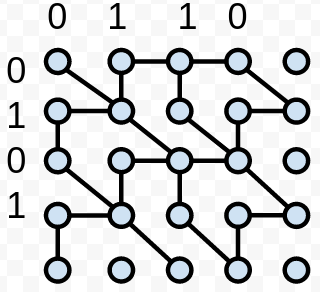
\includegraphics[scale=0.7]{p1_graph.png} \\
Graph of \texttt{0101} and \texttt{0110}.
\columnbreak \\
Because all edges travel in either the positive x, positive y, or positive x and y directions, we know that this graph is acyclic. Because this graph is directed and acyclic, we can use a realtively fast algorithm (compared to the NP-hard algorithm for the longest-path on a general-graph case) to find the longest path. The algorithm contains two parts, making the graph and retreiving the longest path. To find the longest path, we have to find a topological sort of the graph. \\
This can be done with a modifed version of DFS that pushes vertices onto a stack, at the very end that stack will contain the topological sort of G. Once we have this sort, we can find the longest path using a simple algorithm. \\ 
\end{multicols}

Start by walking over all $m \times n$ vertices in the graph and generating edges. Each vertex can have at most two edges eminated from it, so each of the $m \times n$ operation are constant. Thus constructing the graph is $O(mn)$. Once the graph is constructed, DFS is run on it which runs in time $O(|V+E|)$, since $E \leq 2*|V|$, DFS runs in time $O(|V|) = O(mn)$. DFS gives us our topoligical sort, which leads to the last portion of our algorithm, retreiving the longest path. \\
The algorithm in short walks along the topolical sort from the source vertex (which would be $V(0, 0)$ for the shortest-common-subsequence problem), and updates its neighbors where-ever it can by adding its own weight-sum to the weight of the incident edges and setting the neighbors weight-sum to this value. 
\end{homeworkProblem}






%----------------------------------------------------------------------------------------
%   PROBLEM 2
%----------------------------------------------------------------------------------------

\begin{homeworkProblem}

\begin{center}
\begin{tikzpicture}
  \node[draw,circle] (s) {$s$};
  \node[draw,circle] (b) [right=2cm of s] {$b$};
  \node[draw,circle] (c) [right=2cm of b] {$c$};
  \node[draw,circle] (t) [right=2cm of c] {$t$};
  \node (m) at ($(b)!0.5!(c)$) {};
  \node[draw,circle] (a) [above=1.73cm of m] {$a$};
  \node[draw,circle] (d) [below=1.73cm of m] {$d$};
  \draw[-latex] (s) -- (a) node [pos=.6, above left,draw] {6} node [pos=.4,above] {10};
  \draw[-latex] (s) -- (b) node [pos=.5, above] {3} node [pos=.5, below, draw] {3};
  \draw[-latex] (s) -- (d) node [pos=.4, below] {1} node [pos=.6, below left, draw] {1};
  \draw[-latex] (a) -- (b) node [pos=.6, below] {1} node [pos=.4,below right, draw] {1};
  \draw[-latex] (a) -- (c) node [pos=.5, right]{2};
  \draw[-latex] (a) -- (t) node [pos=.4,above]{5} node [pos=.6,above right, draw]{5};
  \draw[-latex] (b) -- (c) node [pos=.5,above]{6} node [pos=.5,below,draw] {5};
  \draw[-latex] (c) -- (t) node [pos=.5,above]{5} node[pos=.5,below,draw]{5};
  \draw[-latex] (d) -- (b) node [pos=.6,below left,draw] {1} node [pos=.5,right] {3};
  \draw[-latex] (d) -- (c) node [pos=.5, right]{3};
  \draw[-latex] (d) -- (t) node [pos=.5,below]{10};
\end{tikzpicture}
\end{center}
\begin{enumerate}
  \item What is the value of this flow? Is this a maximum $(s,t)$ flow in this graph? \\
  \textbf{Answer : } The value for this flow is 10, as there is 10 units leaving the source and 10 units entering the drain. It is \textbf{not} a maximum
  $(s,t)$ flow in this graph, I can find one that gives a flow of 11 by some clever redirection.\\
  s
  \item Find a minimum $s-t$ cut in the flow network pictured  in Figure 7.27[above], and also say what its capacity is. \\
  \textbf{Answer : } The minimum cut that I found is between the two following sets of vertices : $(s, a, b)$ and $(d, c, t)$. If you count the edges going into $t$, you get an incoming flow of 5+2+6+1=14. When you add up the outgoing flows, you get 3. So the total flow between the two cuts is $14-3 =11$, which is the same as the maximum flow I discovered in part A of this problem.\\
\end{enumerate}

\end{homeworkProblem}



\newpage

%----------------------------------------------------------------------------------------
%   PROBLEM 3
%----------------------------------------------------------------------------------------
\begin{homeworkProblem}

\vspace{2mm}
Decide whether you think the following statement is 
true, give a short explanation. If it is false, give a counterexample.
\begin{addmargin}[2em]{0em}
\textit{%
Let G be an arbitrary flow network, with a source s, a sink t, and a positive
integer capacity $c_e$ on every edge e. If f is a maximum s-t flow in G, then f
saturates every edge out of s with flow (i.e., for all edges e out of s, we have
$f(e)=c_e$).}
\end{addmargin}

\textbf{Answer : } This statement is false, all I needed to do to confirm so was to look at a few examples from the textbook. If the above statement was true, it would vatly simplfiy the process of finding the maximum flow, as it would have to be equal to the sum of the capactities of the edges leaving the source $s$. A concrete counter-example is given below. \\

\end{homeworkProblem}


\newpage


%----------------------------------------------------------------------------------------
%   PROBLEM 4
%----------------------------------------------------------------------------------------
\begin{homeworkProblem}

Decide whether you think the following statement is true or false. If it is
true, give a short explanation. If it is false, give a counterexample.
\begin{addmargin}[2em]{0em}
\textit{%
Let G be an arbitrary flow network, with a source s, a sink t, and a positive
integer capacity $c_e$ on every edge e; and let $(A,B)$ be a minimum s-t cut with
respect to these capacities $\{c_e:e\in E\}$. Now suppose we add $1$ to every capacity;
then $(A,B)$ is still a minimum s-t cut with respect to these new capacities
$\{1+c_e:e\in E\}$.
}
\end{addmargin}

\end{homeworkProblem}
\newpage






% %----------------------------------------------------------------------------------------
% %   PROBLEM 5
% %----------------------------------------------------------------------------------------
\begin{homeworkProblem}


\vspace{2mm}
Suppose you are given a direced graph $G=(V,E)$, with a positive integer
capacity $c_e$ on each edge $e$,...
a maximum $s-t$ flow in $G$, defined by a flow value $f_e$ on each edge
\par Now, suppose we pick a specific edge $e^*\in E$ and reduce its capacity
by 1 unit. Show how to find a maximum flow in the resulting capacitated
graph in time $\mathcal{O}(m+n)$, where $m$ is the number of edges in $G$ and $n$ is the
number of nodes.

\textbf{Answer : } Well, to start, we know that if the chosen edge $e$ is not at capacity, then reducing its capacity by one will obviously not effect the max flow, as we didn't change any flow, just reduced the extra capacity of a single 'pipe'. Thus, if the edge isn't saturated, we don't have to do anything to find the max flow and thus we are done immediately. If, however, the given edge is not saturated : \\
If a given edge is not saturated, and we lower its capacity by one, we will need to forward this effect through the system. So take the decreased flow, and extrapolate that change through the inputs and outputs of that edge that had its capacity reduced. Once the effects of this change have propogated, we an iteration of FF algorithm on the new graph.  FF will find an augmenting path and take it if it exists, which will find maximum-flow value for the new graph. \\

Finding if $e$ is saturated can be done easily, propogating the effects of the reduction in capacity means we at most need to look at all $m$ edges in the graph at most. Finally, running a single iteration of the Ford-Fulkerson runs in time $O(m+n)$, thus the total running time of the algorithm is $O(m+n)$.  

\vspace{6mm}


\end{homeworkProblem}

\newpage





% %----------------------------------------------------------------------------------------
% %   PROBLEM 6
% %----------------------------------------------------------------------------------------
\begin{homeworkProblem}


\vspace{2mm}
Professor Adam has two children who, unfortunately, dislike each other. The problem
is so severe that not only do they refuse to walk to school together, but in fact
each one refuses to walk on any block that the other child has stepped on that day.
The children have no problem with their paths crossing at a corner. Fortunately
both the professor's house and the school are on corners, but beyond that he is not
sure if it is going to be possible to send both of his children to the same school.
The professor has a map of his town. Show how to formulate the problem of determining
whether both his children can go to the same school as maximum-flow problem.s

\textbf{Answer : } To start, the house of the professor represent the source node, as it is where the children leave from when they go to school. The sink node is the school, as it absorbs both students. We also know that the school and home are on street corners, which means there are at least two streets to leave the house from and at least 2 streets to arrive at the school from, which means at minimum we know those two nodes work. We then have to determine if we can find two seperate paths that both leave the home and meet up at the school, without ever crossing eachother along the way. To formalize it in terms of our problem, we let each street corner represent a vertex. Both children can be at the same vertex at the same time. The streets represent the edges of our graph, and each edge has a capactity of 1 because it can at most carry only one of the two children. Our task is then to see what the maximum-flow of this graph is. If it is 0 or 1, then both kids with be forced to take the same edge at some point, which means they will walk on the same street which doesn't work. Thus if maximum-flow is $\leq 1$ the boys can't go to the same school. If, however, the maximum flow is $\geq 2$, both students can go to school together since this means there are two paths with unique edges between the home (source) and the school (sink).
\end{homeworkProblem}

\newpage


%----------------------------------------------------------------------------------------

\end{document}